\chapter{Slot Menu:}

The Slot Menu is an important sub-menu of the Grid Page and is used to manipulate slots in a variety of ways.
\\\\
It can be used to clear, copy, paste one or more slots in a row or to configure a slot's chain settings. It also provides an option to rename the current row and provides a quick way to activate or deactivate various Global Chain Modes.
\screenshot{slot_menu.png}
%\fbox{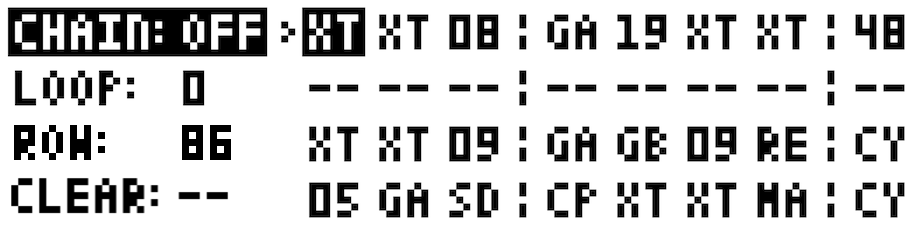
\includegraphics[scale=.40]{slot_menu.png}}\\
\\
\textit{The SlotMenu is accessible from the GridPage by holding down the  \textbf{[Shift2]} function button.\\
\\
When \textbf{[Shift2]} is released, any changes to the menu will be to the selected slots. A rectangular selection consiting of multiple slots can be made by rotating \textbf{[Encoder 1]} and \textbf{[Encoder 2]}. }

\screenshot{range_copy.png}

\section{Slot Menu Options:}
Slot Menu has the following options and selectable values:

\begin{tabular}{|l|l|}
\hline
\rowcolor[HTML]{C0C0C0} 
Entry                                  & Function                                                                                                                                                                                      \\ \hline
Chain: {[} –, auto, manual, random {]} & \begin{tabular}[c]{@{}l@{}}auto: enables chain auto mode global setting.\\ manual: enables chain manual mode global setting.\\ random: enables chain random mode global setting.\end{tabular} \\ \hline
Loops: (0, 64)                         & specify how many times to loop track/slot.                                                                                                                                                    \\ \hline
Row: (0,127)                           & \begin{tabular}[c]{@{}l@{}}specify which row, the current slot is to\\ load/jump to after n loops.\end{tabular}                                                                               \\ \hline

Clear: {[} –, YES {]}                  & clear the selected slot(s).                                                                                                                                                                   \\ \hline
Copy: {[} –, YES {]}                   & copy the selected slot(s).                                                                                                                                                                    \\ \hline
Paste: {[} –, YES {]}                  & paste the selected slot(s).                                                                                                                                                                   \\ \hline
Rename                                 & rename the current row.                                                                                                                                                                       \\ \hline
\end{tabular}

\section{HD44780 LCD users:}
\textit{Note: For users running MCL on a \textbf{HD44780 LCD}, the SlorMenu  is accessible from the GridPage by holding down the  \textbf{[Shift2]} function button and pressing a corresponding encoder button.\\
\\For example if slots 5 to 8 are displayed on screen, holding  \textbf{[Shift2]} and then pressing \textbf{[Encoder3]} will open the slot menu for slot 7.}\\
\\
Rectangular selection is not available for the HD44780. Instead, an additional "APPLY" parameter is provided. If the APPLY value is greater than 1, changes will be applied sequentially; starting from the current slot and up to the number of slots specified by the APPLY value on the same row.

